\problemname{Attention Stones
}

The newest craze to hit the South Pacific is a game called Attention Stones. In Attention Stones, there are $N$ bins labeled 1 to $N$ from left to right. There may be stones in each of the bins. This is a two-player game with alternating turns: Aaron's turn first, then Bertha next, then Aaron, and so on.

On each player's turn, they must find the rightmost nonempty bin (say bin $B$) and select between 1 and $K$ stones, inclusive, from that bin. If that bin was the rightmost bin ($B = N$), then these stones are removed from the game. Otherwise, these stones are placed into bin $B + 1$.

In the example below, if $K=2$, then the player must move either 1 or 2 stones from bin 4 to bin 5. However, if $K=5$, then they may move 1, 2, or all 3 stones from bin 4 to bin 5.

\begin{center}
 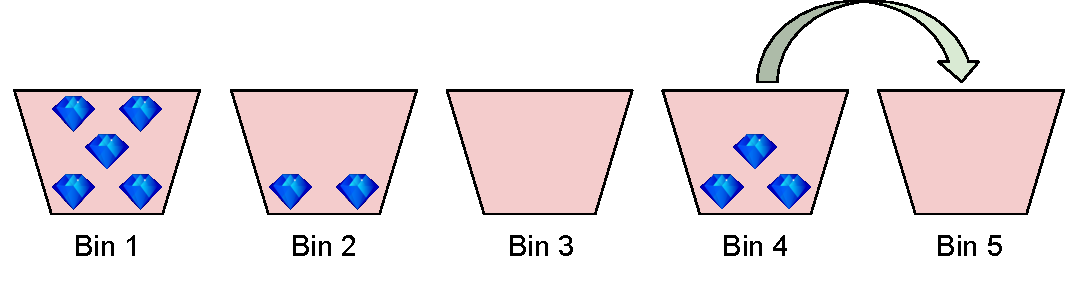
\includegraphics[width=0.6\textwidth]{AttentionStones}
\end{center}

The game is won by the player who removes the final stones from the game. Assuming both players play optimally, who wins?


\section*{Input}

The first line of input contains two integers $N$~($1 \leq N \leq 200\,000$), which is the number of bins, and $K$~($1 \leq K \leq 10^{18}$), which is the maximum number of stones that may be moved on each move.

The next line contains $N$ integers $b_1, b_2, \dots, b_N$~($0 \leq b_i \leq 10^{18}$), which is the number of stones in each bin at the start of the game. There is at least one $i$ such that $b_i > 0$.


\section*{Output}

Display the name of the winner assuming both players play optimally.

